% ========================================================================
% DIAGRAMMES DE PROCESSUS DE CONSTRUCTION
% ========================================================================

\chapter{Modélisation des Processus de Construction}

\begin{objectivebox}
Ce chapitre présente la modélisation complète des processus de construction à travers différents diagrammes : BPMN, flux d'échanges, séquences temporelles et architecture fonctionnelle.
\end{objectivebox}

% ========================================================================
% DIAGRAMME BPMN GLOBAL
% ========================================================================

\section{Diagramme BPMN du Processus de Construction}

\subsection{Vue d'Ensemble du Processus}

Le diagramme BPMN (Business Process Model and Notation) présente une vue complète du processus de construction, depuis la conception jusqu'à la livraison, en incluant tous les acteurs et leurs interactions.

\begin{figure}[H]
\centering
\begin{tikzpicture}[scale=0.7, transform shape]

% Définition des couleurs
\definecolor{maitreouvrage}{HTML}{E8F4FD}
\definecolor{maitreoeuvre}{HTML}{FFF2CC}
\definecolor{entreprise}{HTML}{E1F5FE}
\definecolor{fournisseur}{HTML}{F3E5F5}
\definecolor{administration}{HTML}{E8F5E8}

% Pools (Bassins) - Acteurs principaux
\draw[thick, fill=maitreouvrage] (0,12) rectangle (20,14);
\node[font=\bfseries] at (10,13) {MAÎTRE D'OUVRAGE};

\draw[thick, fill=maitreoeuvre] (0,9) rectangle (20,11.5);
\node[font=\bfseries] at (10,10.25) {MAÎTRE D'ŒUVRE};

\draw[thick, fill=entreprise] (0,6) rectangle (20,8.5);
\node[font=\bfseries] at (10,7.25) {ENTREPRISE DE CONSTRUCTION};

\draw[thick, fill=fournisseur] (0,3) rectangle (20,5.5);
\node[font=\bfseries] at (10,4.25) {FOURNISSEURS};

\draw[thick, fill=administration] (0,0) rectangle (20,2.5);
\node[font=\bfseries] at (10,1.25) {ADMINISTRATION};

% Phase 1: Conception et Planification
\node[draw, circle, fill=green] (start) at (1,13) {\tiny START};
\node[draw, rectangle, rounded corners] (besoin) at (3,13) {\parbox{1.5cm}{\tiny\centering Expression\\du besoin}};
\node[draw, rectangle, rounded corners] (etude) at (3,10.25) {\parbox{1.5cm}{\tiny\centering Étude de\\faisabilité}};
\node[draw, rectangle, rounded corners] (conception) at (5,10.25) {\parbox{1.5cm}{\tiny\centering Conception\\architecturale}};
\node[draw, diamond] (validation1) at (7,10.25) {\tiny OK?};

% Phase 2: Autorisations
\node[draw, rectangle, rounded corners] (permis) at (7,1.25) {\parbox{1.5cm}{\tiny\centering Demande\\permis}};
\node[draw, rectangle, rounded corners] (instruction) at (9,1.25) {\parbox{1.5cm}{\tiny\centering Instruction\\dossier}};
\node[draw, diamond] (accord) at (11,1.25) {\tiny Accordé?};

% Phase 3: Préparation
\node[draw, rectangle, rounded corners] (appel) at (9,7.25) {\parbox{1.5cm}{\tiny\centering Appel\\d'offres}};
\node[draw, rectangle, rounded corners] (selection) at (11,7.25) {\parbox{1.5cm}{\tiny\centering Sélection\\entreprises}};
\node[draw, rectangle, rounded corners] (planning) at (9,10.25) {\parbox{1.5cm}{\tiny\centering Planning\\détaillé}};

% Phase 4: Approvisionnement
\node[draw, rectangle, rounded corners] (consultation) at (9,4.25) {\parbox{1.5cm}{\tiny\centering Consultation\\fournisseurs}};
\node[draw, rectangle, rounded corners] (commande) at (11,4.25) {\parbox{1.5cm}{\tiny\centering Commandes\\matériaux}};
\node[draw, rectangle, rounded corners] (livraison) at (13,4.25) {\parbox{1.5cm}{\tiny\centering Livraisons\\planifiées}};

% Phase 5: Exécution
\node[draw, rectangle, rounded corners] (grosoeuvre) at (13,7.25) {\parbox{1.5cm}{\tiny\centering Gros\\œuvre}};
\node[draw, rectangle, rounded corners] (secondoeuvre) at (15,7.25) {\parbox{1.5cm}{\tiny\centering Second\\œuvre}};
\node[draw, rectangle, rounded corners] (finitions) at (17,7.25) {\parbox{1.5cm}{\tiny\centering Finitions}};

% Phase 6: Contrôle et Livraison
\node[draw, rectangle, rounded corners] (controle) at (15,10.25) {\parbox{1.5cm}{\tiny\centering Contrôles\\qualité}};
\node[draw, rectangle, rounded corners] (reception) at (17,10.25) {\parbox{1.5cm}{\tiny\centering Réception\\travaux}};
\node[draw, rectangle, rounded corners] (livraison_finale) at (17,13) {\parbox{1.5cm}{\tiny\centering Livraison\\finale}};
\node[draw, circle, fill=red] (end) at (19,13) {\tiny END};

% Flèches et flux
\draw[->] (start) -- (besoin);
\draw[->] (besoin) -- (etude);
\draw[->] (etude) -- (conception);
\draw[->] (conception) -- (validation1);
\draw[->] (validation1) -- node[above] {\tiny Oui} (planning);
\draw[->] (validation1) -- node[right] {\tiny Non} (7,8) -- (3,8) -- (etude);

\draw[->] (planning) -- (appel);
\draw[->] (appel) -- (selection);
\draw[->] (selection) -- (grosoeuvre);
\draw[->] (grosoeuvre) -- (secondoeuvre);
\draw[->] (secondoeuvre) -- (finitions);

\draw[->] (conception) -- (7,8) -- (permis);
\draw[->] (permis) -- (instruction);
\draw[->] (instruction) -- (accord);
\draw[->] (accord) -- node[above] {\tiny Oui} (13,1.25) -- (13,6) -- (grosoeuvre);
\draw[->] (accord) -- node[below] {\tiny Non} (7,0.5) -- (permis);

\draw[->] (selection) -- (consultation);
\draw[->] (consultation) -- (commande);
\draw[->] (commande) -- (livraison);
\draw[->] (livraison) -- (13,6) -- (grosoeuvre);

\draw[->] (finitions) -- (controle);
\draw[->] (controle) -- (reception);
\draw[->] (reception) -- (livraison_finale);
\draw[->] (livraison_finale) -- (end);

% Messages entre pools
\draw[dashed, ->] (besoin) -- node[left] {\tiny Cahier des charges} (etude);
\draw[dashed, ->] (planning) -- node[left] {\tiny Plans} (appel);
\draw[dashed, ->] (selection) -- node[left] {\tiny Contrat} (consultation);
\draw[dashed, ->] (finitions) -- node[left] {\tiny Livraison} (controle);

\end{tikzpicture}
\caption{Diagramme BPMN du processus global de construction}
\label{fig:bpmn_construction}
\end{figure}

\subsection{Légende des Éléments BPMN}

\begin{itemize}
    \item \textbf{Pools (Bassins) :} Représentent les acteurs principaux du processus
    \item \textbf{Activités rectangulaires :} Tâches à réaliser par chaque acteur
    \item \textbf{Événements circulaires :} Points de début (vert) et de fin (rouge)
    \item \textbf{Passerelles diamant :} Points de décision avec conditions
    \item \textbf{Flèches continues :} Flux de séquence normal
    \item \textbf{Flèches pointillées :} Messages et échanges entre acteurs
\end{itemize}

% ========================================================================
% DIAGRAMME DE FLUX D'ÉCHANGES
% ========================================================================

\section{Diagramme des Flux d'Échanges}

\subsection{Architecture des Flux Multicouches}

Ce diagramme illustre les différents types de flux qui circulent dans le processus de construction.

\begin{figure}[H]
\centering
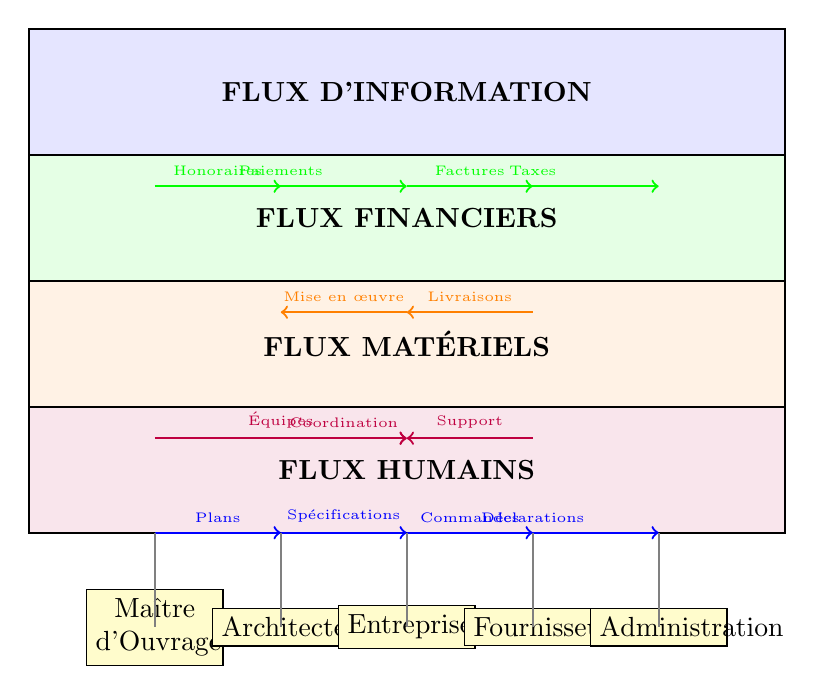
\begin{tikzpicture}[scale=0.8]

% Couches de flux
\draw[thick, fill=blue!10] (0,8) rectangle (12,10);
\node[font=\bfseries] at (6,9) {FLUX D'INFORMATION};

\draw[thick, fill=green!10] (0,6) rectangle (12,8);
\node[font=\bfseries] at (6,7) {FLUX FINANCIERS};

\draw[thick, fill=orange!10] (0,4) rectangle (12,6);
\node[font=\bfseries] at (6,5) {FLUX MATÉRIELS};

\draw[thick, fill=purple!10] (0,2) rectangle (12,4);
\node[font=\bfseries] at (6,3) {FLUX HUMAINS};

% Acteurs connectés
\node[draw, rectangle, fill=yellow!20] (mo) at (2,0.5) {\parbox{1.5cm}{\centering Maître\\d'Ouvrage}};
\node[draw, rectangle, fill=yellow!20] (arch) at (4,0.5) {\parbox{1.5cm}{\centering Architecte}};
\node[draw, rectangle, fill=yellow!20] (entr) at (6,0.5) {\parbox{1.5cm}{\centering Entreprise}};
\node[draw, rectangle, fill=yellow!20] (fourn) at (8,0.5) {\parbox{1.5cm}{\centering Fournisseur}};
\node[draw, rectangle, fill=yellow!20] (admin) at (10,0.5) {\parbox{1.5cm}{\centering Administration}};

% Flux d'information (bleu)
\draw[thick, blue, ->] (2,2) -- node[above] {\tiny Plans} (4,2);
\draw[thick, blue, ->] (4,2) -- node[above] {\tiny Spécifications} (6,2);
\draw[thick, blue, ->] (6,2) -- node[above] {\tiny Commandes} (8,2);
\draw[thick, blue, ->] (6,2) -- node[above] {\tiny Déclarations} (10,2);

% Flux financiers (vert)
\draw[thick, green, ->] (2,7.5) -- node[above] {\tiny Honoraires} (4,7.5);
\draw[thick, green, ->] (2,7.5) -- node[above] {\tiny Paiements} (6,7.5);
\draw[thick, green, ->] (6,7.5) -- node[above] {\tiny Factures} (8,7.5);
\draw[thick, green, ->] (6,7.5) -- node[above] {\tiny Taxes} (10,7.5);

% Flux matériels (orange)
\draw[thick, orange, ->] (8,5.5) -- node[above] {\tiny Livraisons} (6,5.5);
\draw[thick, orange, ->] (6,5.5) -- node[above] {\tiny Mise en œuvre} (4,5.5);

% Flux humains (violet)
\draw[thick, purple, ->] (2,3.5) -- node[above] {\tiny Équipes} (6,3.5);
\draw[thick, purple, ->] (4,3.5) -- node[above] {\tiny Coordination} (6,3.5);
\draw[thick, purple, ->] (8,3.5) -- node[above] {\tiny Support} (6,3.5);

% Connexions vers acteurs
\foreach \x in {2,4,6,8,10} {
    \draw[thick, gray] (\x,2) -- (\x,0.5);
}

\end{tikzpicture}
\caption{Architecture des flux multicouches dans la construction}
\label{fig:flux_multicouches}
\end{figure}

\subsection{Types de Flux Détaillés}

\subsubsection{Flux d'Information}
\begin{itemize}
    \item \textbf{Descendants :} Plans, spécifications, instructions, budgets
    \item \textbf{Ascendants :} Rapports d'avancement, comptes-rendus, alertes
    \item \textbf{Horizontaux :} Coordination inter-métiers, partage de plans
\end{itemize}

\subsubsection{Flux Financiers}
\begin{itemize}
    \item \textbf{Entrants :} Versements clients, financements, subventions
    \item \textbf{Sortants :} Paiements fournisseurs, salaires, frais de fonctionnement
\end{itemize}

\subsubsection{Flux Matériels}
\begin{itemize}
    \item \textbf{Approvisionnement :} Livraisons, transport, stockage, contrôle qualité
    \item \textbf{Utilisation :} Distribution, transformation, gestion des déchets
\end{itemize}

\subsubsection{Flux Humains}
\begin{itemize}
    \item \textbf{Mobilisation :} Recrutement, formation, coordination
    \item \textbf{Gestion :} Planning des équipes, gestion des compétences
\end{itemize}

% ========================================================================
% DIAGRAMME DE SÉQUENCE - PROCESSUS D'ESTIMATION
% ========================================================================

\section{Diagramme de Séquence - Processus d'Estimation}

\subsection{Interactions Temporelles pour l'Estimation IA}

Ce diagramme présente les interactions séquentielles lors du processus d'estimation avec intelligence artificielle.

\begin{figure}[H]
\centering
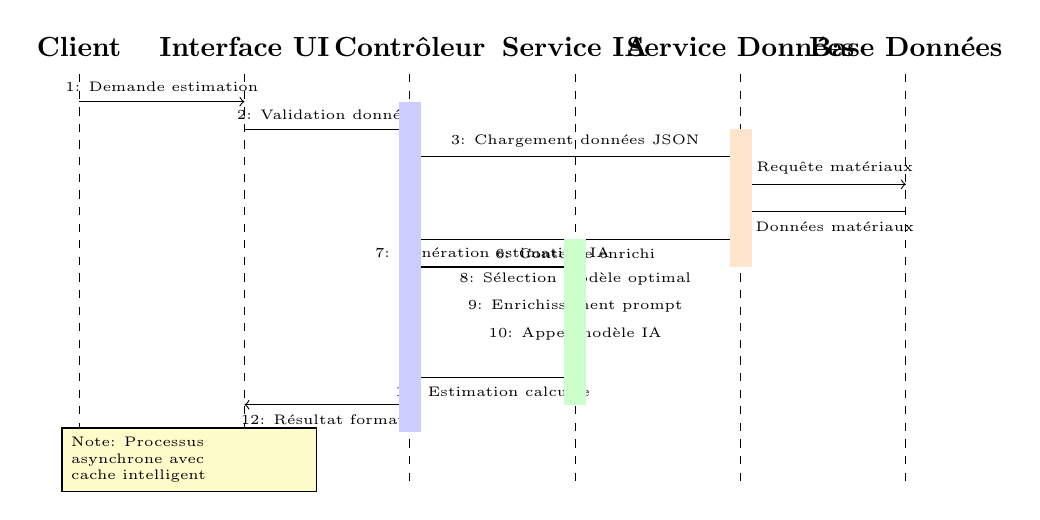
\begin{tikzpicture}[scale=0.7]

% Acteurs
\node (client) at (0,8) {\textbf{Client}};
\node (ui) at (3,8) {\textbf{Interface UI}};
\node (controller) at (6,8) {\textbf{Contrôleur}};
\node (aiservice) at (9,8) {\textbf{Service IA}};
\node (dataservice) at (12,8) {\textbf{Service Données}};
\node (db) at (15,8) {\textbf{Base Données}};

% Lignes de vie
\foreach \x in {0,3,6,9,12,15} {
    \draw[dashed] (\x,7.5) -- (\x,0);
}

% Messages et interactions
\draw[->] (0,7) -- node[above] {\tiny 1: Demande estimation} (3,7);
\draw[->] (3,6.5) -- node[above] {\tiny 2: Validation données} (6,6.5);
\draw[->] (6,6) -- node[above] {\tiny 3: Chargement données JSON} (12,6);
\draw[->] (12,5.5) -- node[above] {\tiny 4: Requête matériaux} (15,5.5);
\draw[<-] (12,5) -- node[below] {\tiny 5: Données matériaux} (15,5);
\draw[<-] (6,4.5) -- node[below] {\tiny 6: Contexte enrichi} (12,4.5);

\draw[->] (6,4) -- node[above] {\tiny 7: Génération estimation IA} (9,4);
\draw[->] (9,3.5) -- node[above] {\tiny 8: Sélection modèle optimal} (9,3.5);
\draw[->] (9,3) -- node[above] {\tiny 9: Enrichissement prompt} (9,3);
\draw[->] (9,2.5) -- node[above] {\tiny 10: Appel modèle IA} (9,2.5);

\draw[<-] (6,2) -- node[below] {\tiny 11: Estimation calculée} (9,2);
\draw[<-] (3,1.5) -- node[below] {\tiny 12: Résultat formaté} (6,1.5);
\draw[<-] (0,1) -- node[below] {\tiny 13: Affichage estimation} (3,1);

% Zones d'activation
\fill[blue!20] (5.8,7) rectangle (6.2,1);
\fill[green!20] (8.8,4.5) rectangle (9.2,1.5);
\fill[orange!20] (11.8,6.5) rectangle (12.2,4);

% Notes explicatives
\node[draw, rectangle, fill=yellow!20] at (2,0.5) {\parbox{3cm}{\tiny Note: Processus\\asynchrone avec\\cache intelligent}};

\end{tikzpicture}
\caption{Diagramme de séquence du processus d'estimation IA}
\label{fig:sequence_estimation}
\end{figure}

\subsection{Étapes Détaillées du Processus}

\begin{enumerate}
    \item \textbf{Demande initiale :} L'utilisateur saisit les paramètres du projet
    \item \textbf{Validation :} Contrôle de cohérence des données d'entrée
    \item \textbf{Chargement contexte :} Récupération des données JSON de référence
    \item \textbf{Enrichissement :} Injection des données réelles dans le prompt
    \item \textbf{Sélection IA :} Choix du modèle optimal selon l'utilisateur
    \item \textbf{Génération :} Calcul de l'estimation par l'intelligence artificielle
    \item \textbf{Formatage :} Mise en forme des résultats pour l'affichage
    \item \textbf{Retour utilisateur :} Présentation de l'estimation détaillée
\end{enumerate}

% ========================================================================
% DIAGRAMME D'ACTIVITÉ - VALIDATION DE PROJET
% ========================================================================

\section{Diagramme d'Activité - Processus de Validation}

\subsection{Workflow de Validation des Projets}

Ce diagramme illustre le processus de validation et d'approbation des projets de construction.

\begin{figure}[H]
\centering
\begin{tikzpicture}[scale=0.6]

% Début
\node[draw, circle, fill=green] (start) at (2,12) {\tiny START};

% Activités séquentielles
\node[draw, rectangle, rounded corners] (soumission) at (2,10.5) {\parbox{2.5cm}{\centering Soumission\\du projet}};
\node[draw, rectangle, rounded corners] (verification) at (2,9) {\parbox{2.5cm}{\centering Vérification\\complétude}};

% Point de décision 1
\node[draw, diamond] (complet) at (2,7.5) {\parbox{1.5cm}{\centering Dossier\\complet?}};

% Branche non-conforme
\node[draw, rectangle, rounded corners] (retour1) at (6,7.5) {\parbox{2.5cm}{\centering Demande\\compléments}};

% Validation technique
\node[draw, rectangle, rounded corners] (validation_tech) at (2,6) {\parbox{2.5cm}{\centering Validation\\technique}};

% Activités parallèles
\node[draw, rectangle, rounded corners] (verif_normes) at (0,4.5) {\parbox{2cm}{\centering Vérification\\normes}};
\node[draw, rectangle, rounded corners] (verif_budget) at (4,4.5) {\parbox{2cm}{\centering Vérification\\budget}};

% Point de synchronisation
\node[draw, rectangle, thick] (sync1) at (2,3) {};

% Point de décision 2
\node[draw, diamond] (conforme) at (2,1.5) {\parbox{1.5cm}{\centering Projet\\conforme?}};

% Branche rejet
\node[draw, rectangle, rounded corners] (rejet) at (6,1.5) {\parbox{2.5cm}{\centering Notification\\rejet}};
\node[draw, circle, fill=red] (end_rejet) at (6,0) {\tiny END};

% Approbation finale
\node[draw, rectangle, rounded corners] (approbation) at (2,0) {\parbox{2.5cm}{\centering Approbation\\finale}};
\node[draw, circle, fill=green] (end_ok) at (2,-1.5) {\tiny END};

% Flèches et flux
\draw[->] (start) -- (soumission);
\draw[->] (soumission) -- (verification);
\draw[->] (verification) -- (complet);
\draw[->] (complet) -- node[left] {\tiny Non} (retour1);
\draw[->] (retour1) -- (6,9) -- (soumission);
\draw[->] (complet) -- node[left] {\tiny Oui} (validation_tech);

% Fork vers activités parallèles
\draw[->] (validation_tech) -- (2,5) -- (0,5) -- (verif_normes);
\draw[->] (2,5) -- (4,5) -- (verif_budget);

% Join des activités parallèles
\draw[->] (verif_normes) -- (0,3) -- (sync1);
\draw[->] (verif_budget) -- (4,3) -- (sync1);
\draw[->] (sync1) -- (conforme);

\draw[->] (conforme) -- node[right] {\tiny Non} (rejet);
\draw[->] (rejet) -- (end_rejet);
\draw[->] (conforme) -- node[left] {\tiny Oui} (approbation);
\draw[->] (approbation) -- (end_ok);

% Zones de responsabilité
\draw[dashed, blue] (-1,11.5) rectangle (5,5.5);
\node[blue] at (6.5,8.5) {\parbox{2cm}{\tiny Zone\\Chef de\\Projet}};

\draw[dashed, red] (-1,5.5) rectangle (5,-2);
\node[red] at (6.5,2) {\parbox{2cm}{\tiny Zone\\Validation\\Technique}};

\end{tikzpicture}
\caption{Diagramme d'activité du processus de validation}
\label{fig:activite_validation}
\end{figure}

\subsection{Éléments du Workflow}

\begin{itemize}
    \item \textbf{Activités séquentielles :} Soumission, vérification, validation
    \item \textbf{Activités parallèles :} Vérification normes et budget simultanées
    \item \textbf{Points de décision :} Contrôles de conformité avec conditions
    \item \textbf{Zones de responsabilité :} Délimitation des rôles et permissions
    \item \textbf{Gestion d'exceptions :} Processus de retour et correction
\end{itemize}

% ========================================================================
% ARCHITECTURE FONCTIONNELLE HOUSY
% ========================================================================

\section{Architecture Fonctionnelle de Housy Tunisia}

\subsection{Vue d'Ensemble de l'Architecture}

Cette section présente l'architecture technique de la solution Housy Tunisia avec ses différentes couches et composants.

\begin{figure}[H]
\centering
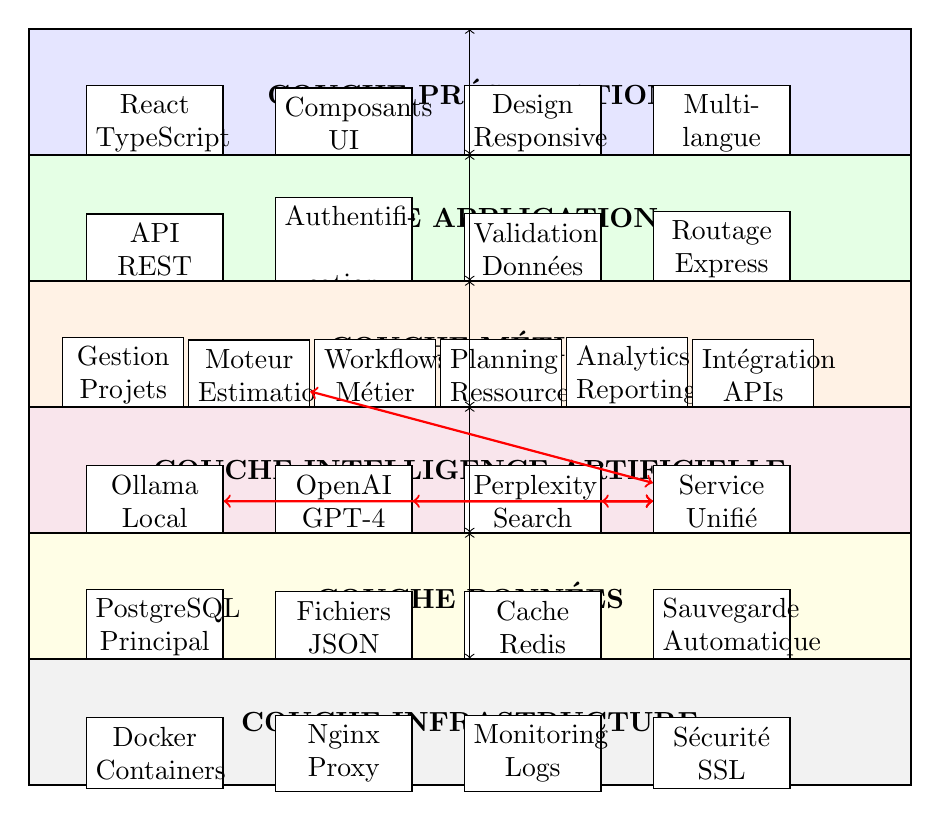
\begin{tikzpicture}[scale=0.8]

% Couche Présentation
\draw[thick, fill=blue!10] (0,10) rectangle (14,12);
\node[font=\bfseries] at (7,11) {COUCHE PRÉSENTATION};

\node[draw, rectangle, fill=white] (react) at (2,10.5) {\parbox{1.5cm}{\centering React\\TypeScript}};
\node[draw, rectangle, fill=white] (components) at (5,10.5) {\parbox{1.5cm}{\centering Composants\\UI}};
\node[draw, rectangle, fill=white] (responsive) at (8,10.5) {\parbox{1.5cm}{\centering Design\\Responsive}};
\node[draw, rectangle, fill=white] (i18n) at (11,10.5) {\parbox{1.5cm}{\centering Multi-\\langue}};

% Couche Application
\draw[thick, fill=green!10] (0,8) rectangle (14,10);
\node[font=\bfseries] at (7,9) {COUCHE APPLICATION};

\node[draw, rectangle, fill=white] (api) at (2,8.5) {\parbox{1.5cm}{\centering API\\REST}};
\node[draw, rectangle, fill=white] (auth) at (5,8.5) {\parbox{1.5cm}{\centering Authentifi-\\cation}};
\node[draw, rectangle, fill=white] (validation) at (8,8.5) {\parbox{1.5cm}{\centering Validation\\Données}};
\node[draw, rectangle, fill=white] (routing) at (11,8.5) {\parbox{1.5cm}{\centering Routage\\Express}};

% Couche Métier
\draw[thick, fill=orange!10] (0,6) rectangle (14,8);
\node[font=\bfseries] at (7,7) {COUCHE MÉTIER};

\node[draw, rectangle, fill=white] (projects) at (1.5,6.5) {\parbox{1.3cm}{\centering Gestion\\Projets}};
\node[draw, rectangle, fill=white] (estimation) at (3.5,6.5) {\parbox{1.3cm}{\centering Moteur\\Estimation}};
\node[draw, rectangle, fill=white] (workflow) at (5.5,6.5) {\parbox{1.3cm}{\centering Workflows\\Métier}};
\node[draw, rectangle, fill=white] (planning) at (7.5,6.5) {\parbox{1.3cm}{\centering Planning\\Ressources}};
\node[draw, rectangle, fill=white] (reporting) at (9.5,6.5) {\parbox{1.3cm}{\centering Analytics\\Reporting}};
\node[draw, rectangle, fill=white] (integration) at (11.5,6.5) {\parbox{1.3cm}{\centering Intégration\\APIs}};

% Couche Intelligence Artificielle
\draw[thick, fill=purple!10] (0,4) rectangle (14,6);
\node[font=\bfseries] at (7,5) {COUCHE INTELLIGENCE ARTIFICIELLE};

\node[draw, rectangle, fill=white] (ollama) at (2,4.5) {\parbox{1.5cm}{\centering Ollama\\Local}};
\node[draw, rectangle, fill=white] (openai) at (5,4.5) {\parbox{1.5cm}{\centering OpenAI\\GPT-4}};
\node[draw, rectangle, fill=white] (perplexity) at (8,4.5) {\parbox{1.5cm}{\centering Perplexity\\Search}};
\node[draw, rectangle, fill=white] (unified) at (11,4.5) {\parbox{1.5cm}{\centering Service\\Unifié}};

% Couche Données
\draw[thick, fill=yellow!10] (0,2) rectangle (14,4);
\node[font=\bfseries] at (7,3) {COUCHE DONNÉES};

\node[draw, rectangle, fill=white] (postgresql) at (2,2.5) {\parbox{1.5cm}{\centering PostgreSQL\\Principal}};
\node[draw, rectangle, fill=white] (json) at (5,2.5) {\parbox{1.5cm}{\centering Fichiers\\JSON}};
\node[draw, rectangle, fill=white] (cache) at (8,2.5) {\parbox{1.5cm}{\centering Cache\\Redis}};
\node[draw, rectangle, fill=white] (backup) at (11,2.5) {\parbox{1.5cm}{\centering Sauvegarde\\Automatique}};

% Couche Infrastructure
\draw[thick, fill=gray!10] (0,0) rectangle (14,2);
\node[font=\bfseries] at (7,1) {COUCHE INFRASTRUCTURE};

\node[draw, rectangle, fill=white] (docker) at (2,0.5) {\parbox{1.5cm}{\centering Docker\\Containers}};
\node[draw, rectangle, fill=white] (nginx) at (5,0.5) {\parbox{1.5cm}{\centering Nginx\\Proxy}};
\node[draw, rectangle, fill=white] (monitoring) at (8,0.5) {\parbox{1.5cm}{\centering Monitoring\\Logs}};
\node[draw, rectangle, fill=white] (security) at (11,0.5) {\parbox{1.5cm}{\centering Sécurité\\SSL}};

% Connexions entre couches
\foreach \y in {2,4,6,8,10} {
    \draw[<->] (7,\y) -- (7,\y+2);
}

% Connexions spécifiques IA
\draw[<->, red, thick] (estimation) -- (unified);
\draw[<->, red, thick] (unified) -- (ollama);
\draw[<->, red, thick] (unified) -- (openai);
\draw[<->, red, thick] (unified) -- (perplexity);

\end{tikzpicture}
\caption{Architecture technique multicouche de Housy Tunisia}
\label{fig:architecture_technique}
\end{figure}

\subsection{Description des Couches}

\subsubsection{Couche Présentation}
\begin{itemize}
    \item \textbf{React/TypeScript :} Framework moderne pour interface utilisateur
    \item \textbf{Composants UI :} Bibliothèque de composants réutilisables
    \item \textbf{Design Responsive :} Adaptation mobile et desktop
    \item \textbf{Multi-langue :} Support français et arabe
\end{itemize}

\subsubsection{Couche Application}
\begin{itemize}
    \item \textbf{API REST :} Interface standardisée pour communications
    \item \textbf{Authentification :} Gestion sécurisée des utilisateurs
    \item \textbf{Validation :} Contrôle d'intégrité des données
    \item \textbf{Routage :} Gestion des endpoints et middleware
\end{itemize}

\subsubsection{Couche Métier}
\begin{itemize}
    \item \textbf{Gestion Projets :} CRUD et workflow des projets
    \item \textbf{Moteur Estimation :} Calculs intelligents avec IA
    \item \textbf{Workflows :} Processus métier automatisés
    \item \textbf{Planning :} Gestion des ressources et planning
    \item \textbf{Analytics :} Tableaux de bord et KPI
    \item \textbf{Intégrations :} APIs externes et partenaires
\end{itemize}

\subsubsection{Couche Intelligence Artificielle}
\begin{itemize}
    \item \textbf{Ollama Local :} Modèles IA locaux (Qwen, Llama)
    \item \textbf{OpenAI :} GPT-4 Turbo pour précision maximale
    \item \textbf{Perplexity :} Recherche en temps réel
    \item \textbf{Service Unifié :} Orchestration intelligente des modèles
\end{itemize}

\subsubsection{Couche Données}
\begin{itemize}
    \item \textbf{PostgreSQL :} Base de données relationnelle principale
    \item \textbf{Fichiers JSON :} Référentiels métier (matériaux, prix)
    \item \textbf{Cache Redis :} Performance et mise en cache
    \item \textbf{Sauvegarde :} Stratégie de backup automatisée
\end{itemize}

\subsubsection{Couche Infrastructure}
\begin{itemize}
    \item \textbf{Docker :} Containerisation et portabilité
    \item \textbf{Nginx :} Reverse proxy et load balancing
    \item \textbf{Monitoring :} Surveillance système et logs
    \item \textbf{Sécurité :} Chiffrement SSL et protection
\end{itemize}

% ========================================================================
% CONCLUSION DU CHAPITRE
% ========================================================================

\section{Conclusion}

\subsection{Synthèse de la Modélisation}

Ce chapitre a présenté une modélisation complète du processus de construction à travers plusieurs approches complémentaires :

\begin{enumerate}
    \item \textbf{BPMN Global :} Vue d'ensemble du processus avec tous les acteurs
    \item \textbf{Flux Multicouches :} Analyse détaillée des échanges
    \item \textbf{Séquences Temporelles :} Interactions précises pour l'estimation IA
    \item \textbf{Workflows Métier :} Processus de validation et approbation
    \item \textbf{Architecture Technique :} Structure de la solution Housy
\end{enumerate}

\subsection{Apports de la Modélisation}

\begin{itemize}
    \item \textbf{Compréhension globale :} Vision claire du processus complexe
    \item \textbf{Identification des flux :} Optimisation des échanges
    \item \textbf{Points d'amélioration :} Digitalisation ciblée des processus
    \item \textbf{Architecture cohérente :} Solution technique adaptée
\end{itemize}

\subsection{Transition vers l'Implémentation}

Cette modélisation constitue la base de l'implémentation technique de Housy Tunisia, garantissant :
\begin{itemize}
    \item Respect des processus métier existants
    \item Optimisation par la digitalisation
    \item Architecture évolutive et maintenable
    \item Intégration harmonieuse de l'intelligence artificielle
\end{itemize}

\begin{resultbox}
La modélisation complète du processus de construction fournit une base solide pour le développement de Housy Tunisia, assurant une solution parfaitement adaptée aux besoins du secteur tunisien.
\end{resultbox}

\end{tikzpicture}
